\chapter{Navržené blokové zapojení reflektometru}
V předchozích kapitolách byly vysvětleny technologie, které byly uvažovány pro návrh architektury jednoduchého reflektometru a následně byly z nich vybrány ty nejvhodnější nebo nejjednodušší na implementaci. Pro jednotlivé části reflektometru tedy budou použity tyto stavební bloky:
\begin{itemize}
	\item
	\textbf{Buzení}\\*
	Pro buzení bude použito buzení aproximovaným jednotkovým skokem pomocí budiče technologie \acrshort{CML}, kterým je možné dosáhnout aproximace s náběžnou hranou o délce kratší než \SI{100}{\pico\second}, typicky okolo \SI{60}{\pico\second}, tedy s užitečnou šířkou pásma v jednotkách \si{\giga\hertz}. Výstup je dobře přizpůsoben pro použití v \SI{50}{\ohm} systémech.
	
	\item
	\textbf{Separace budicího a odraženého signálu}\\*	
	Pro separaci buzení od odezvy systému bude použito prodlužovací vedení jako metoda pro dosažení časového posunu. Samotná separace bude probíhat až z navzorkovaných dat během zpracování.
	
	\item
	\textbf{Vzorkování}\\*	
	Data budou sbírána pomocí postupného vzorkování v ekvivalentním čase pomocí vyvážených diodových můstků. Touto metodou je možné vzorkovat měřený signál pomocí pomalých převodníků s větším dynamickým rozsahem a přesností, je také možné potlačit ruchy z okolí. Byla navržena metoda pro měření s dynamickým rozsahem nejméně \SI{80}{\deci\bel}.
	
	\item
	\textbf{Generování signálů pro řízení reflektometru}\\*	
	Pro řízení jednotlivých částí reflektometru bude použita \acrshort{PLL} Si5351, která disponuje 8 výstupy, které je možné konfigurovat jako diferenciální výstupy. Jednotlivé výstupy mohou mít neceločíselné vzájemné poměry frekvencí (krok nastavení je menší než \SI{1}{ppm}), je možné dosáhnout vzorkování s krokem menším než \SI{100}{\pico\second}, tedy ekvivalentní vzorkovací frekvence větší než \SI{10}{\gigasample}. Díky proudovým výstupům je možné ji přímo propojit jak se vstupy \acrshort{CML} logických prvků, tak ji použít pro spínání diodových vzorkovačů. Je možné i vygenerovat synchronizační hodinový signál pro mikrokontrolér, aby se provádělo vzorkování v přesně stanovený čas.
\end{itemize}

Z těchto jednotlivých prvků je tedy již možné navrhnout základní blokové zapojení navrhované architektury. Toto blokové zapojení je na obrázku \ref{reflectometer_blockdiagram}.

\begin{figure}[htbp]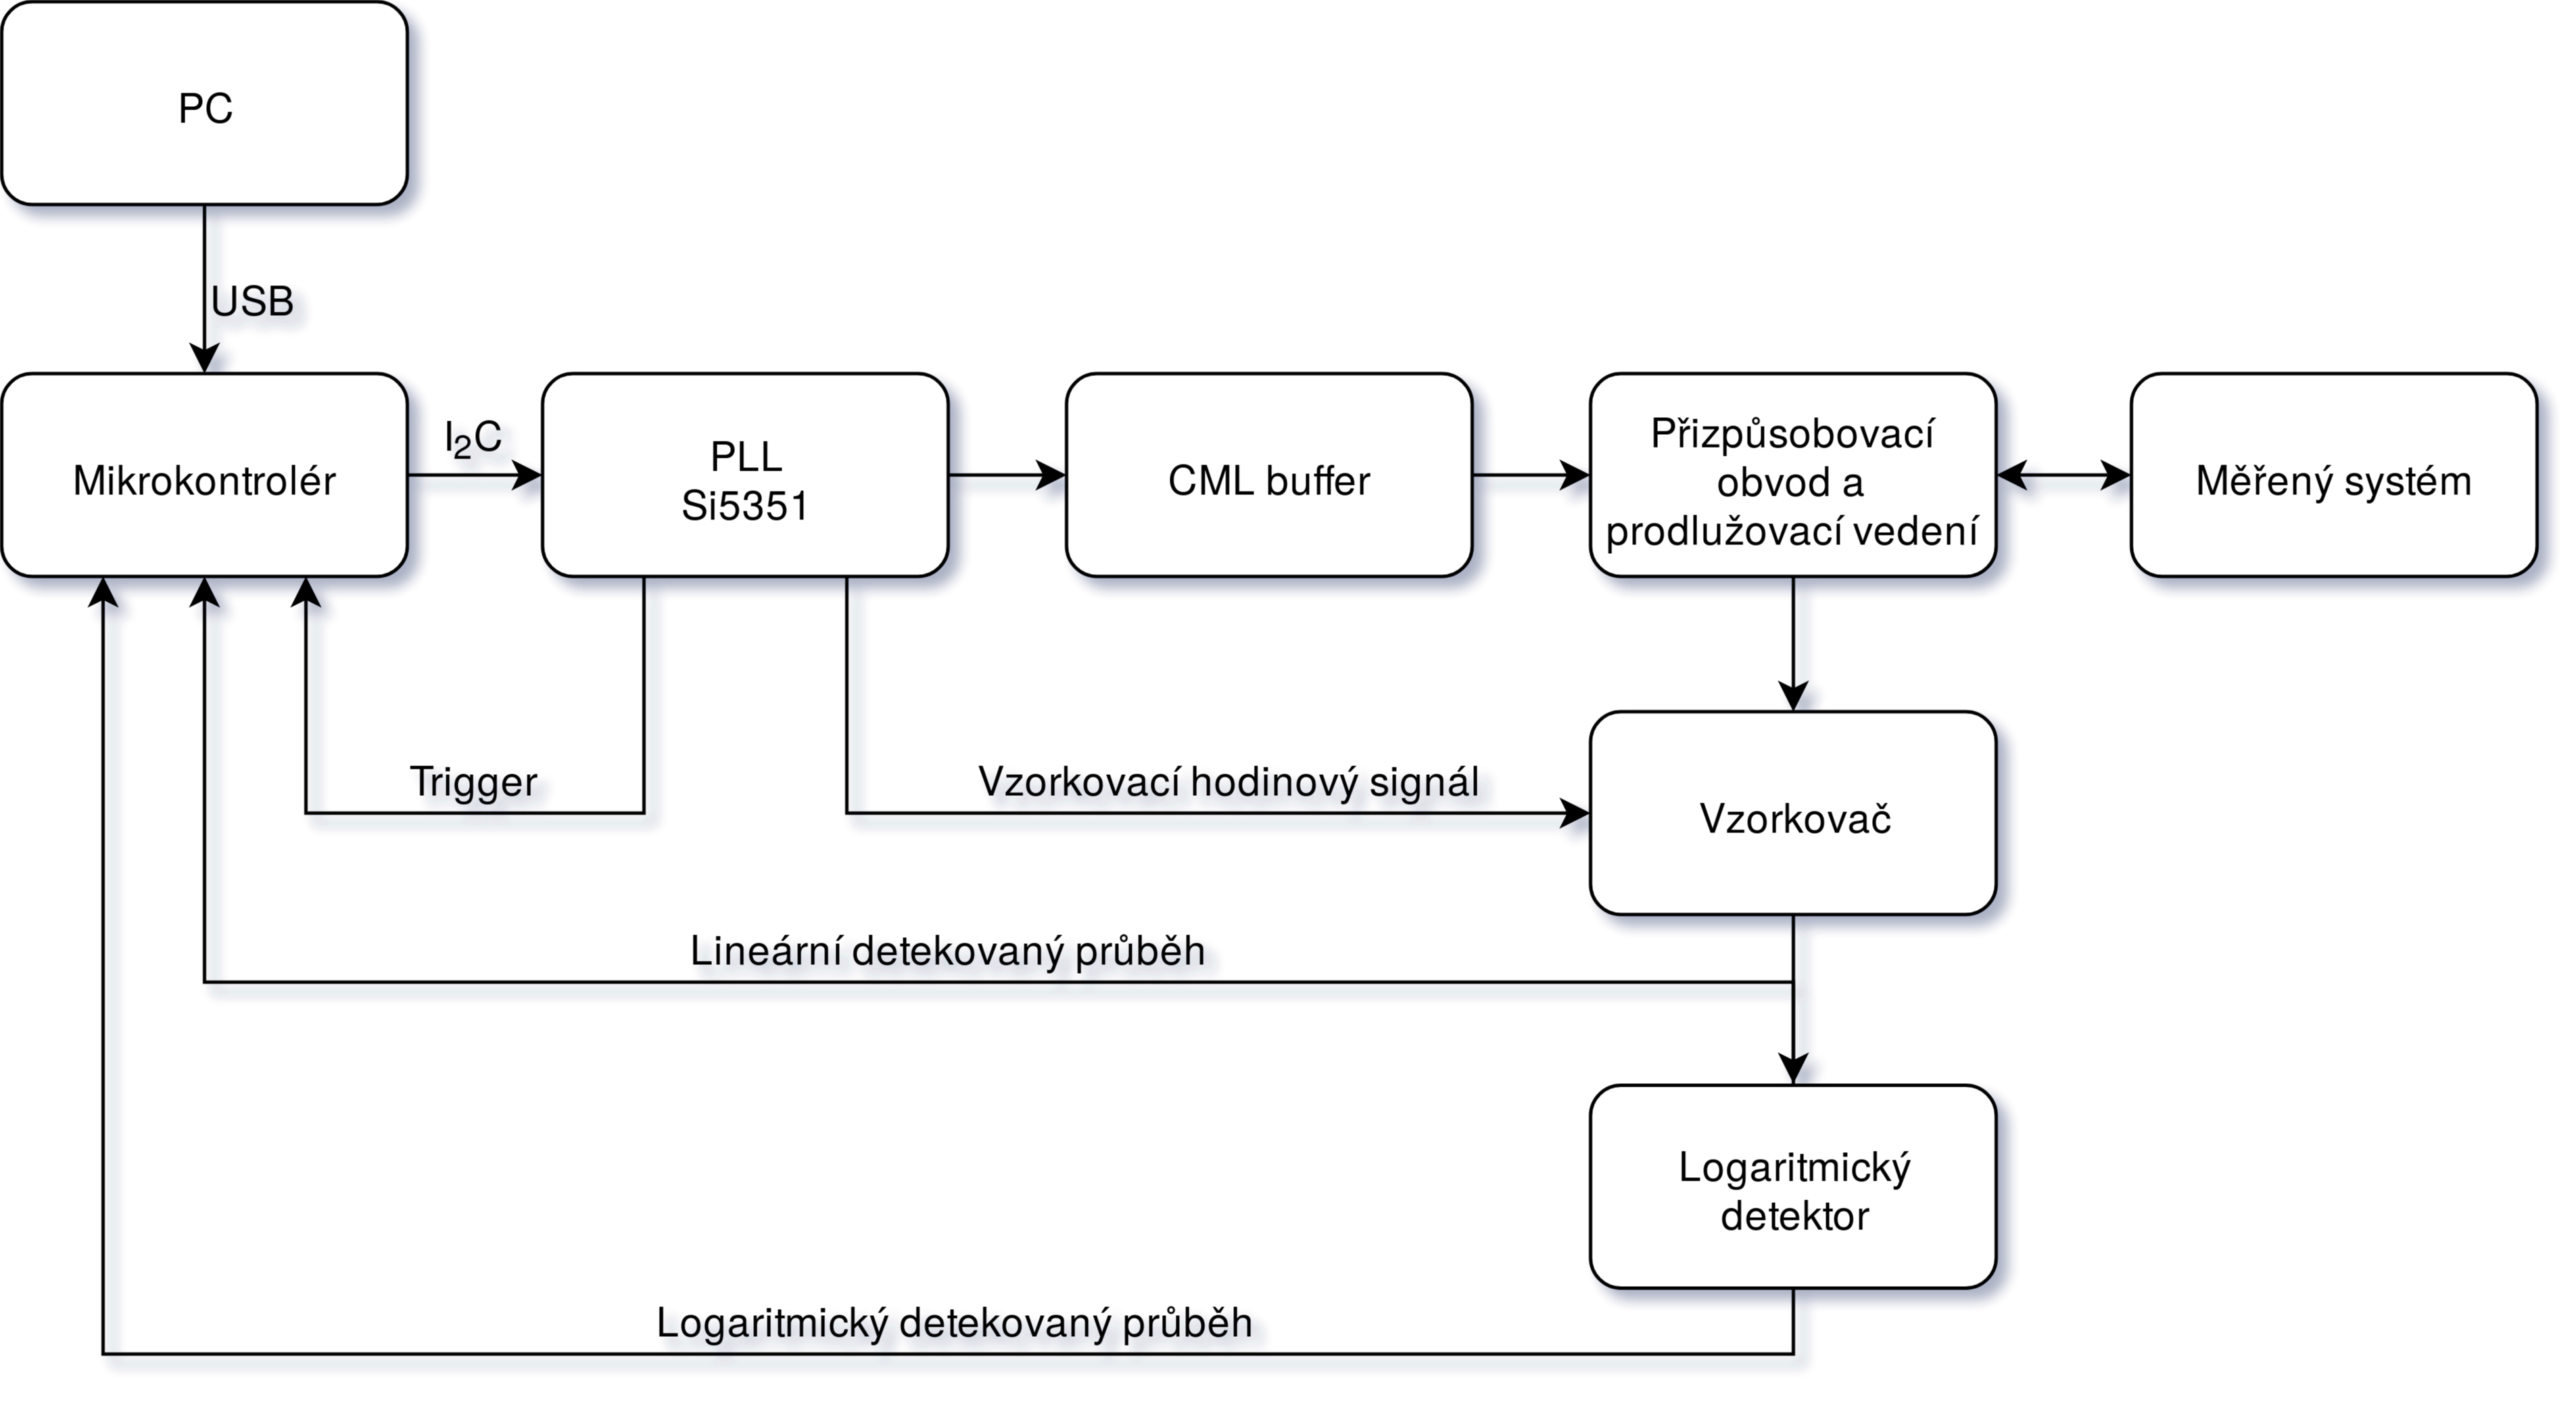
\includegraphics[width=\textwidth,keepaspectratio]{images/reflectometer_blockdiagram_simple.png}\caption{Základní blokové schéma navržené architektury reflektometru.}\label{reflectometer_blockdiagram}\end{figure}